\section{java.util.Map}

\frame{\frametitle{java.util.Map}
\begin{center}
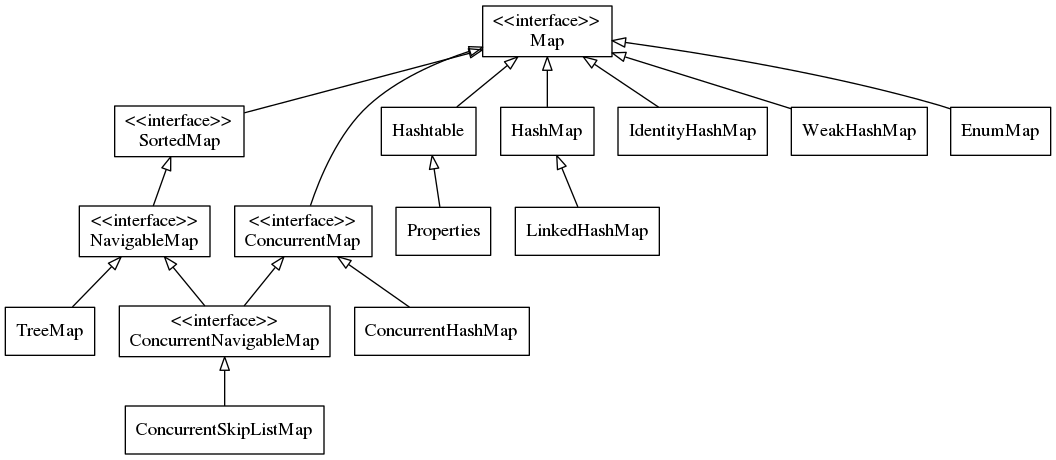
\includegraphics[width=0.9\textwidth]{java.util.Map/java_util_Map_overview}
\end{center}
}

%%%%%%%%%%%%%%%%%
%    HashMap    %
%%%%%%%%%%%%%%%%%

\frame{
\frametitle{HashMap}
\begin{center}
  \begin{itemize}[<+->]
    \item seit 1.2
    \item null keys und values erlaubt
    \item wie Hashtable, aber mit nulls und nicht thread-safe
    \item get/put in \O{1}
    \item nicht thread-safe
    \item fail-fast iterator
  \end{itemize}
\end{center}
}

\begin{frame}[fragile]
\frametitle{HashMap - interne Struktur}
\begin{itemize}[<+->]
  \item capacity = Anzahl an buckets, initialCapacity = Start capacity
  \item loadFactor = Ab wann automatisch rehash
  \item rehash: interne Datenstruktur wird neu gebaut $\Rightarrow$ Kapazität steigt um Faktor 2
  \item Konstruktor: initialCapacity und loadFactor \\
	$DEFAULT_LOAD_FACTOR = 0.75f$ \\
	$DEFAULT_INITIAL_CAPACITY = 1 << 4; // = 16$
  \item wenn $number\ entries \geq loadFactor * capacity$ dann rehash
  \item wenn viele puts, dann sollte initialCapacity groß genug sein, um Anzahl an rehashes klein zu halten
  \item aber initialCapacity nicht zu hoch und loadFactor nicht zu niedrig setzen, sonst zu viele rehashes
\end{itemize}
\end{frame}

\frame{
\frametitle{HashMap - Zugriffszeiten}
\begin{center}
  \begin{tabular}{l|l}
  Operation        & Laufzeit \\\hline
  get              & \O{1} \\
  put              & \O{1} \\
  \end{tabular}
\end{center}
}

\frame{
\frametitle{HashMap - Wann nehmen?}
\begin{center}
  Synchronisation egal, \\\pause
  Ordnung egal, \\\pause
  oft get/put
\end{center}
}


%%%%%%%%%%%%%%%%%
% LinkedHashMap %
%%%%%%%%%%%%%%%%%


\frame{
\frametitle{LinkedHashMap}
\begin{center}
  \begin{itemize}[<+->]
    \item null erlaubt
    \item add, contains, remove \O{1}
    \item iteration = \O{size}, HashMap = \O{capacity}, schneller falls $size < capacity$
    \item initial capacity and load factor wie HashMap
    \item not synchronized, nicht thread-safe
    \item fail-fast iterator
    \item Reihenfolge nach Einfügen (insertion-order)
  \end{itemize}
\end{center}
}

\begin{frame}[fragile]
\frametitle{LinkedHashMap - LRU-Cache}
  \begin{block}{Least Recently Used}
    \begin{enumerate}[<+->]
      \item \textit{new LinkedHashMap(initialCapacity, loadFactor, accessOrder)} \\
	    accessOrder = true für access-order, von least nach most-recently \\
      \item um nach put / putAll zu aktualisieren removeEldestEntry überschreiben
	  \begin{lstlisting}
     @Override
     protected boolean removeEldestEntry(Map.Entry eldest) {
        return size() > 100;
     }
	  \end{lstlisting}
    \end{enumerate}
  \end{block}
\end{frame}

\frame{
\frametitle{LinkedHashMap - Zugriffszeiten}
\begin{center}
  \begin{tabular}{l|l}
  Operation        & Laufzeit \\\hline
  add              & \O{1} \\
  contains         & \O{1} \\
  remove           & \O{1} \\
  get              & \O{TODO} \\
  put              & \O{TODO} \\
  \end{tabular}
\end{center}
}

\frame{
\frametitle{LinkedHashMap - Wann nehmen?}
\begin{center}
  Reihenfolge wichtig oder \\\pause
  schnelle Iteration (schneller als HashMap)
\end{center}
}


%%%%%%%%%%%%%%%%%%%%
% IdentityHashMap  %
%%%%%%%%%%%%%%%%%%%%

\frame{
\frametitle{IdentityHashMap}
\begin{center}
  \begin{itemize}[<+->]
    \item hashed mit System.identityHashCode(Object) anstatt der hashCode Implementierung
    \item Referenz-Gleichheit anstatt equals \\
	  \textit{if (k1==k2)} anstatt \\
	  \textit{if (k1==null ? k2==null : k1.equals(k2))} (HashMap)
    \item betrifft nur keys
    \item verletzt bewusst den Map-Vertrag ''equals() zum Vergleichen''
    \item null keys/values erlaubt
    \item keine Reihenfolge
    \item get/put in O(1)
    \item expected maximum size sollte genutzt werden, erweitern ist teuer
    \item nicht thread-safe
    \item fail-fast iterator
  \end{itemize}
\end{center}
}

\frame{
\frametitle{IdentityHashMap - Wann nehmen?}
\begin{center}
  nur wenn Referenz-Gleichheit gebraucht wird (sehr selten)
\end{center}
}


%%%%%%%%%%%%%%%%%%%%
%   WeakHashMap    %
%%%%%%%%%%%%%%%%%%%%

\frame{
\frametitle{WeakHashMap}
\begin{center}
  \begin{itemize}[<+->]
    \item ...
  \end{itemize}
\end{center}
}


%%%%%%%%%%%%%%%%%%%%%
% ConcurrentHashMap %
%%%%%%%%%%%%%%%%%%%%%

\frame{
\frametitle{ConcurrentHashMap}
\begin{center}
  \begin{itemize}[<+->]
    \item ...
  \end{itemize}
\end{center}
}


%%%%%%%%%%%%%%%%%%%%
%      EnumMap     %
%%%%%%%%%%%%%%%%%%%%

\frame{
\frametitle{EnumMap}
\begin{center}
  \begin{itemize}[<+->]
    \item ...
  \end{itemize}
\end{center}
}


%%%%%%%%%%%%%%%%%
%   Hashtable   %
%%%%%%%%%%%%%%%%%

\frame{
\frametitle{Hashtable}
\begin{center}
  \begin{itemize}[<+->]
    \item ...
  \end{itemize}
\end{center}
}


%%%%%%%%%%%%%%%%%
%   Properties  %
%%%%%%%%%%%%%%%%%

\frame{
\frametitle{Properties}
\begin{center}
  \begin{itemize}[<+->]
    \item ...
  \end{itemize}
\end{center}
}


%%%%%%%%%%%%%%%%%
%    TreeMap    %
%%%%%%%%%%%%%%%%%

\frame{
\frametitle{TreeMap}
\begin{center}
  \begin{itemize}[<+->]
    \item ...
  \end{itemize}
\end{center}
}


%%%%%%%%%%%%%%%%%%%%%%%%%
% ConcurrentSkipListMap %
%%%%%%%%%%%%%%%%%%%%%%%%%

\frame{
\frametitle{ConcurrentSkipListMap}
\begin{center}
  \begin{itemize}[<+->]
    \item ...
  \end{itemize}
\end{center}
}


%%%%%%%%%%%%%%%%%%%%%%%%%
%       Übersicht       %
%%%%%%%%%%%%%%%%%%%%%%%%%

\frame{
\frametitle{Map - Übersicht}
\begin{center}
  \begin{tabular}{l|c|c|c|c}
                        & thread-safe &  Iterator &    Reihenfolge     & null value \\\hline
  HashMap               &     nein    & fail-fast &                    &   erlaubt  \\
  LinkedHashMap         &     nein    & fail-fast & insertion / access &   erlaubt  \\
  IdentityHashMap       &     nein    & fail-fast &                    &   erlaubt  \\
  WeakHashMap           &             &           &                    &            \\
  ConcurrentHashMap     &             &           &                    &            \\
  EnumMap               &             &           &                    &            \\
  Hashtable             &             &           &                    &            \\
  Properties            &             &           &                    &            \\
  TreeMap               &             &           &                    &            \\
  ConcurrentSkipListMap &             &           &                    &            \\
  \end{tabular}
\end{center}
}
